\subsection{Wechselspannung}
    \vspace{-1em}
    \begin{align*}
        \parbox{4cm}{\textbf{Komplexe Schreibweise:}}\\
        \overset{\sim}{I}(t) = I_0 e^{i \omega t}, \quad \overset{\sim}{U} &= \overset{\sim}{Z} \cdot \overset{\sim}{I} = I_0 Z \cdot e^{i \omega t} e^{i \rho}
        \\[0.5em]
        \parbox{4cm}{\textbf{Impedanz Spule:}}\\
        \overset{\sim}{Z}_S = R + i \omega L &= \sqrt{R^2 + \omega^2 L ^2} \cdot e^{i \rho}\\
        \text{Phasenverschiebung $\rho$:} \; U(t) &\sim I(t + \frac{\pi}{2})
        \\[0.5em]
        \parbox{4cm}{\textbf{Impedanz Kondensator:}}\\
        \overset{\sim}{Z}_C = - i\frac{1}{\omega C} &= \frac{1}{\omega C} \cdot e^{i \rho}\\
        \text{Phasenverschiebung $\rho$:} \; U(t) &\sim I(t - \frac{\pi}{2})
        \\[0.5em]
        \parbox{4cm}{\textbf{Impedanz Widerstand:}}\\
        \overset{\sim}{Z}_R = R &= R \cdot e^{i \rho}\\
        \text{Phasenverschiebung $\rho$:} \; U(t) &\sim I(t)
        \\[0.5em]
        \parbox{4cm}{\textbf{Leistung:}}\\
        P = \frac{1}{2} I_0 U_0 cos(\rho)\\
        \parbox{4cm}{\textbf{Winkel Phasenverschiebung im Schaltkreis:}}\\
        \tan(\Phi) = \frac{|Z_L| - |Z_C|}{Z_R}
    \end{align*}

    \tikzset{
        pattern size/.store in=\mcSize, 
        pattern size = 5pt,
        pattern thickness/.store in=\mcThickness, 
        pattern thickness = 0.3pt,
        pattern radius/.store in=\mcRadius, 
        pattern radius = 1pt}
        \makeatletter
        \pgfutil@ifundefined{pgf@pattern@name@_9395wxxuh}{
        \pgfdeclarepatternformonly[\mcThickness,\mcSize]{_9395wxxuh}
        {\pgfqpoint{-\mcThickness}{-\mcThickness}}
        {\pgfpoint{\mcSize}{\mcSize}}
        {\pgfpoint{\mcSize}{\mcSize}}
        {
        \pgfsetcolor{\tikz@pattern@color}
        \pgfsetlinewidth{\mcThickness}
        \pgfpathmoveto{\pgfpointorigin}
        \pgfpathlineto{\pgfpoint{0}{\mcSize}}
        \pgfusepath{stroke}
    }}
    \makeatother
    % Pattern Info
    \tikzset{
        pattern size/.store in=\mcSize, 
        pattern size = 5pt,
        pattern thickness/.store in=\mcThickness, 
        pattern thickness = 0.3pt,
        pattern radius/.store in=\mcRadius, 
        pattern radius = 1pt}
        \makeatletter
        \pgfutil@ifundefined{pgf@pattern@name@_r1aowurqw}{
        \pgfdeclarepatternformonly[\mcThickness,\mcSize]{_r1aowurqw}
        {\pgfqpoint{-\mcThickness}{-\mcThickness}}
        {\pgfpoint{\mcSize}{\mcSize}}
        {\pgfpoint{\mcSize}{\mcSize}}
        {
        \pgfsetcolor{\tikz@pattern@color}
        \pgfsetlinewidth{\mcThickness}
        \pgfpathmoveto{\pgfpointorigin}
        \pgfpathlineto{\pgfpoint{0}{\mcSize}}
        \pgfusepath{stroke}
    }}
    \makeatother
    \tikzset{every picture/.style={line width=0.75pt}} %set default line width to 0.75pt        

    \begin{center} 
        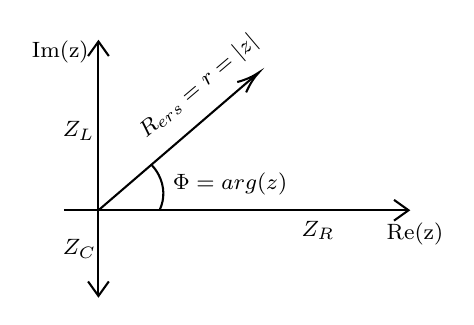
\begin{tikzpicture}[x=0.75pt,y=0.75pt,yscale=-1,xscale=1]
            %uncomment if require: \path (0,209); %set diagram left start at 0, and has height of 209
            % R_ers
            \draw (58.6,109.3) -- (134.1,44.4) ; % Line R_ers
            \draw [shift={(135.9,42.9)}, rotate = 139.32] [color={rgb, 255:red, 0; green, 0; blue, 0 }  ][line width=0.75]    (10.93,-3.29) .. controls (6.95,-1.4) and (3.31,-0.3) .. (0,0) .. controls (3.31,0.3) and (6.95,1.4) .. (10.93,3.29)   ; % Arrowhead R_ers
            \draw (74.22,68.61) node [anchor=north west][inner sep=0.75pt]  [font=\footnotesize,rotate=-319.68]  {$R_{\text{ers}} = r = |z|$}; % Text Node R_ers

            % Z_R
            \draw (42,109.3) -- (208,109.3); % Line Z_R
            \draw (201,104.3) -- (208,109.3) -- (201,114.3); % Arrowhead Z_R
            \draw (196,114) node [anchor=north west][inner sep=0.75pt]  [font=\footnotesize] [align=left] {Re(z)}; % Text Node Re(z)
            \draw (155,113) node [anchor=north west][inner sep=0.75pt]  [font=\footnotesize]  {$Z_R$}; % Text Node Z_R
            
            % Z_L
            \draw (58.6,28) -- (58.6,109.3); % Line Z_L
            \draw (53.6,35) -- (58.6,28) -- (63.6,35); % Arrowhead Z_L
            \draw (25,26) node [anchor=north west][inner sep=0.75pt]  [font=\footnotesize] [align=left] {Im(z)}; % Text Node Im(z)
            \draw (40,65) node [anchor=north west][inner sep=0.75pt]  [font=\footnotesize]  {$Z_L$}; % Text Node Z_L

            % Z_C
            \draw (58.6,109.3) -- (58.6,150.6); % Line Z_C
            \draw (53.6,143.6) -- (58.6,150.6) -- (63.6,143.6); % Arrowhead Z_C
            \draw (40,122) node [anchor=north west][inner sep=0.75pt]  [font=\footnotesize]  {$Z_C$}; %Text Node Z_C

            % Phi
            %\draw (83.87,147.15) .. controls (85.33,148.6) and (86.59,150.28) .. (87.58,152.18) .. controls (90.53,157.77) and (90.52,163.98) .. (88.13,169.06) -- (70.36,160.23) -- cycle ;
            \draw (83.87,87.15) .. controls (85.33,88.6) and (86.59,90.28) .. (87.58,92.18) .. controls (90.53,97.77) and (90.52,103.98) .. (88.13,109.06) ; % Angle Phi
            \draw (93,90) node [anchor=north west][inner sep=0.75pt]  [font=\footnotesize]  {$\Phi=\text{arg}(z)$};
        \end{tikzpicture}
    \end{center}

    % Spule: 
    % \mathbox{U_L = L \frac{dI}{dt}}

    % Kondensator:
    % \mathbox{U_C = \frac{1}{C} \int I(t) dt}

    % Impedanz:
    % \mathbox{Z_{\text{tot}} = \sum_i Z_i, \frac{1}{Z_{\text{tot}}} = \sum_i \frac{}{Z_i}}